\documentclass[ paper=a4
              % , pagesize
              , fontsize=12pt
              , twoside=true
              , bibliography=totoc
              , index=totoc
              , version=last
              ]{scrbook}
\usepackage[all,2cell]{xy}\UseAllTwocells
\usepackage{itaca}
\usepackage{quiver}
\usetikzlibrary{intersections}
\usetikzlibrary{shapes.geometric, positioning, fit}
\recalctypearea
\makeindex
%%% debug area
\tracinglostchars=3  % Increase verbosity
\errorcontextlines=10 % Show more context around errors
%%%

\begin{document}
% \begin{center}
 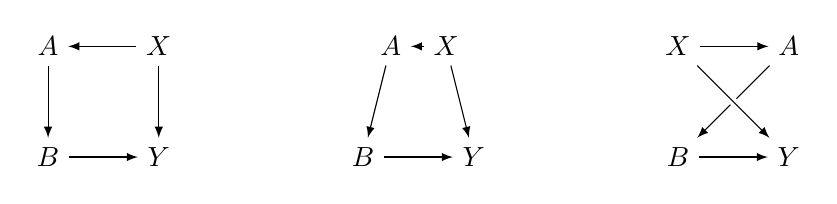
\begin{tikzpicture}[
   x=4em, y=4em,
   dot/.style={
     circle,
     fill=#1,
     inner sep=0pt,
     outer sep=2pt,
     minimum size=4pt,
     draw=none,
    },
   wrap/.style={
     fill=black!5,
     draw=gray,
     rounded corners,
     inner sep=.5em,
    },
  ]

\node (A) at (0,0) {$A$};
\node (B) at (0,-1) {$B$};
\node (X) at (1,0) {$X$};
\node (Y) at (1,-1) {$Y$};
\draw[-latex] (A) -- (B);
\draw[-latex] (X) -- (Y);
\draw[-latex] (B) -- (Y);
\draw[-latex] (X) -- (A);
\begin{scope}[xshift=4cm]
\node (A) at (.25,0) {$A$};
\node (B) at (0,-1) {$B$};
\node (X) at (.75,0) {$X$};
\node (Y) at (1,-1) {$Y$};
\draw[-latex] (A) -- (B);
\draw[-latex] (X) -- (Y);
\draw[-latex] (B) -- (Y);
\draw[-latex] (X) -- (A);
\end{scope}
\begin{scope}[xshift=8cm]
\node (A) at (1,0) {$A$};
\node (B) at (0,-1) {$B$};
\node (X) at (0,0) {$X$};
\node (Y) at (1,-1) {$Y$};
\draw[-latex] (A) -- (B);
\draw[-latex] (B) -- (Y);
\draw[-latex] (X) -- (A);
\draw[line width=3pt,white,-] (X) -- (Y);
\draw[-latex] (X) -- (Y);
\end{scope}
\end{tikzpicture}
\end{document}
